\documentclass[
12pt,
openright,
oneside,
a4paper,
chapter=TITLE,
english,
brazil,
table
]{abntex2}

\usepackage{cmap}				% Mapear caracteres especiais no PDF
\usepackage[utf8]{inputenc} 			% utf8 definition
\usepackage[T1]{fontenc}                        % Isso arruma o problema de copiar/colar do PDF em alguns programas. Tbm dá pra usar '<' e '>'.
\usepackage{lastpage}          			% Usado pela Ficha catalográfica
\usepackage{indentfirst} 			% Primeiro paragrafo tbm é identado
\usepackage{color}				% Controle das cores
\usepackage{mathptmx} 				% usar fonte Times new Roman
\usepackage{xcolor} 				% Pacote para cores na tabela
\usepackage{blindtext}				% Lorem ipsum

% identacao de paragrafo
\setlength{\parindent}{1.25cm}

% fonte dos títulos dos chapters agora é bold
\renewcommand{\ABNTEXchapterfont}{\fontseries{b}}
\renewcommand{\ABNTEXsectionfont}{\fontseries{m}}
\renewcommand{\ABNTEXsubsectionfont}{\fontseries{m}}
\renewcommand{\ABNTEXsubsubsectionfont}{\fontseries{m}}

% tamanho 12 pra todos os títulos
\renewcommand{\ABNTEXchapterfontsize}{\normalsize}
\renewcommand{\ABNTEXsectionfontsize}{\normalsize}
\renewcommand{\ABNTEXsubsectionfontsize}{\normalsize}
\renewcommand{\ABNTEXsubsubsectionfontsize}{\normalsize}

% image usage configuration
\usepackage{graphicx}
\graphicspath{{imagens/}}

\usepackage[brazilian,hyperpageref]{backref}	 				% Paginas com as citações na bibl
\usepackage[alf,abnt-full-initials=yes,abnt-title-command=yes]{abntex2cite}	% Citações padrão ABNT

\makeatletter\AtBeginDocument{\let\@elt\relax}\makeatother

% Change the way to make a reference to a text
\renewcommand{\backref}{}
\renewcommand*{\backrefalt}[4]{
	\ifcase #1
		Nenhuma citação no texto.
	  	\or
		Citado na página #2.
	\else
		Citado #1 vezes nas páginas #2.
\fi}

\providecommand\imprimircurso{\erro\curso}
\newcommand*\curso[1]{\renewcommand{\imprimircurso}{#1}}

\providecommand\imprimirpalavraschave{\erro\palavraschave}
\newcommand*\palavraschave[1]{\renewcommand{\imprimirpalavraschave}{#1}}

% definir erro de definição
\newcommand*\erro[1]{\@latex@error{Defina \noexpand#1!}\@ehc}

\autor{Nome do autor}
\curso{Nome do curso}
\data{Ano}
\local{Cidade}
\instituicao{Nome da universidade}
\orientador{Orientador}
\palavraschave{Palavras chave}
\preambulo{Explicação do trabalho}
\tipotrabalho{Tipo do trabalho}
\titulo{Titulo do trabalho}


\renewcommand{\imprimircapa}{
	\begin{capa}
	\center
	{\large\MakeUppercase\imprimirinstituicao}\par
	{\large\MakeUppercase\imprimircurso}\par
	\vfill
	{\large\MakeUppercase\imprimirautor}\par
	\vfill
	{\bfseries\large\MakeUppercase\imprimirtitulo}\par
	\vfill
		\vfill
		{\large\MakeUppercase\imprimirlocal}\par
	{\large\imprimirdata}\par
	\end{capa}
}

\renewcommand{\imprimirfolhaderosto}{
	\begin{capa}
	\center
	{\large\MakeUppercase\imprimirautor}\par
	\vfill
	{\bfseries\large\MakeUppercase\imprimirtitulo}\par
	\vspace{10 mm}
	\hspace{.45\textwidth}
	\begin{minipage}{.5\textwidth}
	\SingleSpacing
		\imprimirpreambulo
		\\
		\\
		\imprimirorientadorRotulo

		{\large  } \large\imprimirorientador\par
	\end{minipage}
	\vfill
		\vfill
		{\large\MakeUppercase\imprimirlocal}\par
	{\large\imprimirdata}\par
	\end{capa}
}


\makeatletter
\hypersetup{
pdftitle={\@title},
pdfauthor={\@author},
pdfsubject={\imprimirpreambulo},
pdfkeywords={\imprimirpalavraschave},
pdfcreator={LaTeX with abnTeX2},
% make links have color
% colorlinks=true,
% linkcolor=blue,
% citecolor=blue,
% urlcolor=blue
}
\makeatother


\newcommand{\bibtextitlecommand}[2]{\textbf{#2}}

\begin{document}

\frenchspacing
\imprimircapa
\imprimirfolhaderosto
\clearpage

\begin{fichacatalografica}
  \sffamily
  \vspace*{\fill}					% Posição vertical
  \begin{center}					% Minipage Centralizado
    \fbox{\begin{minipage}[c][8cm]{13.5cm}		% Largura
        \small
        \imprimirautor

        \hspace{0.5cm}
        \imprimirtitulo

        \hspace{0.5cm}
        \imprimirlocal, \imprimirdata

        \hspace{0.5cm} \thelastpage p. : il. (algumas color.) ; 30 cm.\\

        \hspace{0.5cm} \imprimirorientadorRotulo~\imprimirorientador\\

        \hspace{0.5cm}
        \parbox[t]{\textwidth}{\imprimirtipotrabalho~--~\imprimirinstituicao,
        \imprimirdata.}\\

        \hspace{0.5cm}
        \imprimirpalavraschave
    \end{minipage}}
  \end{center}
\end{fichacatalografica}

\begin{folhadeaprovacao}

  \begin{center}
    {\ABNTEXchapterfont\large\imprimirautor}

    \vspace*{\fill}\vspace*{\fill}
    \begin{center}
      \ABNTEXchapterfont\bfseries\Large\imprimirtitulo
    \end{center}
    \vspace*{\fill}

    \hspace{.45\textwidth}
    \begin{minipage}{.5\textwidth}
      \imprimirpreambulo
    \end{minipage}%
    \vspace*{\fill}
  \end{center}

  Trabalho aprovado. \imprimirlocal, X de Y de \imprimirdata:

  \assinatura{\textbf{\imprimirorientador} \\ Orientador}
  \assinatura{\textbf{Professor} \\ Convidado 1}

  \begin{center}
    \vspace*{0.5cm}
    {\large\imprimirlocal}
    \par
    {\large\imprimirdata}
    \vspace*{1cm}
  \end{center}

\end{folhadeaprovacao}

\begin{agradecimentos}

  \blindtext

\end{agradecimentos}

\begin{epigrafe}
  \vspace*{\fill}
  \begin{flushright}
    \textit{``Frase inspiradora``.\\
    (Autor)}
  \end{flushright}
\end{epigrafe}

\begin{resumo}

  \blindtext

  \textbf{Palavras chave}: \imprimirpalavraschave

\end{resumo}

\begin{resumo}[Abstract]

  \blindtext

  \textbf{Keywords}: \imprimirpalavraschave

\end{resumo}


\pdfbookmark[0]{\listfigurename}{lof}
\listoffigures*
\cleardoublepage

\pdfbookmark[0]{\listtablename}{lot}
\listoftables*
\cleardoublepage

\begin{siglas}
  \item[ABNT] Associação Brasileira de Normas Técnicas
  \item[abnTeX] Normas ABNT para TeX
\end{siglas}

\begin{simbolos}
  \item[$ \Lambda $] Lambda
\end{simbolos}


\pdfbookmark[0]{\contentsname}{toc}
\tableofcontents*
\cleardoublepage

\textual

\chapter{Intrudução}

\blindtext

\chapter{Objetivo}

\blindtext


\chapter{Fundamentos teoricos}

\blindtext

\chapter{Trabalhos relacionados}

\blindtext

\chapter{Desenvolvimento}

\blindtext

\begin{figure}[h]
	\centering
	\caption{Foto de exemplo}
	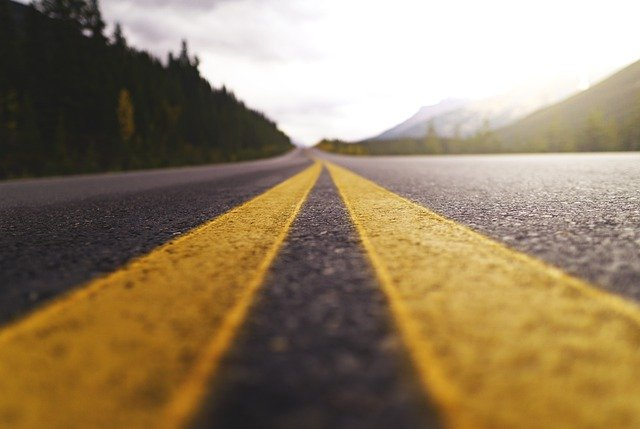
\includegraphics[width=0.88\textwidth]{exemplo}
	\label{fig:exemplo}
	\fonte{\cite{exemplo_img}}
\end{figure}

\section{Subcapítulos}
\blindenumerate[10]

\section{Outro subcapítulos}
\blindtext[5]


\bibliography{referencias}

\end{document}
